\documentclass[12pt]{report}
\usepackage{caption}
\usepackage{graphicx}
\usepackage{hyperref}
\hypersetup{%
    pdfborder = {0 0 0}
}
\hypersetup{
    colorlinks,
    citecolor=blue,
    filecolor=blue,
    linkcolor=blue,
    urlcolor=blue
}
\renewcommand{\familydefault}{\sfdefault}
\renewcommand{\captionfont}{\small}

\author{Bernd Porr}
\title{Realtime embedded coding under Linux}

\begin{document}

\maketitle

\tableofcontents

\chapter{Writing C++ device driver classes}

\begin{figure}[!hbt]
\begin{center}
\mbox{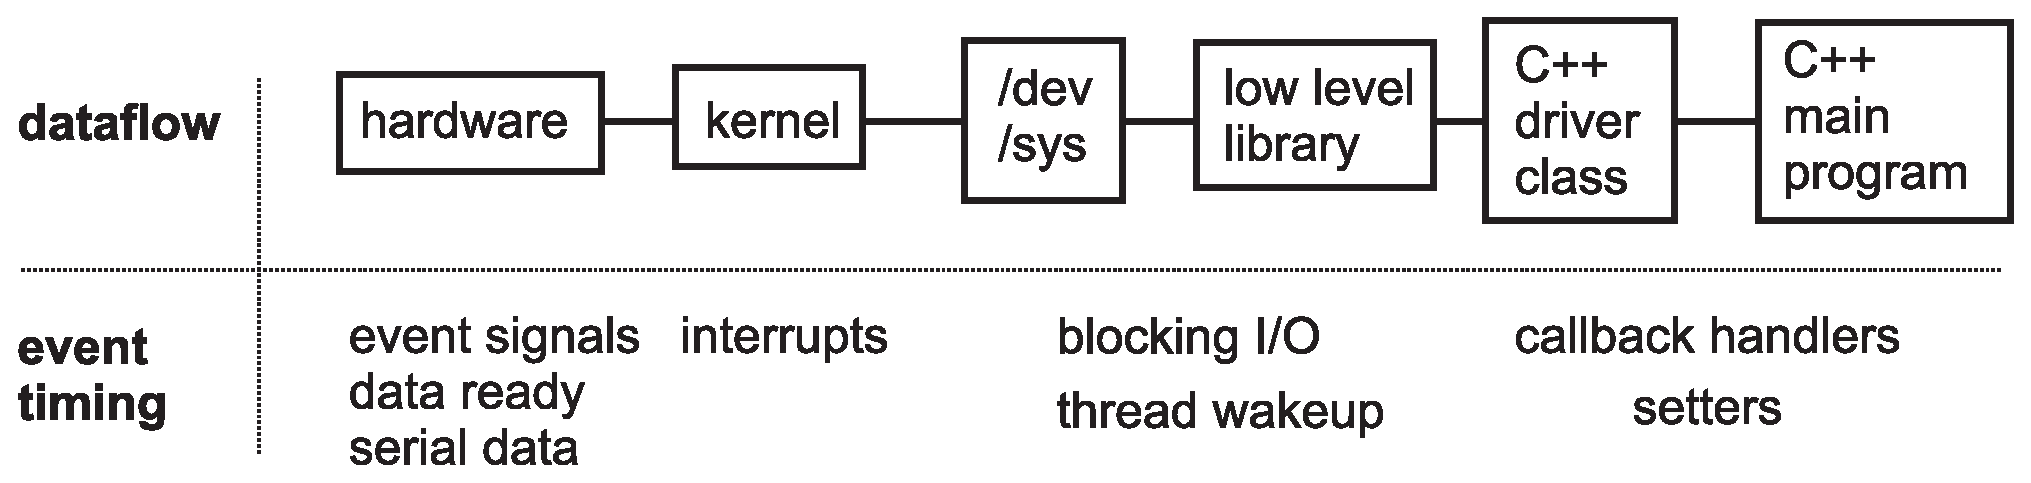
\includegraphics[width=\textwidth]{signals-timings}}
\end{center}
\caption{Dataflow and timing in low level realtime coding
\label{timing}}
\end{figure}

\section{Introduction}
Fig.~\ref{timing} shows the basic dataflow and how event timing
is established. While it's obvious that data needs to flow
from/to the hardware it's even more important to guarantee
its timing. On the hardware-side the timing is guaranteed
by event signals, data-ready signals and also by the timing
of a serial interface. The Linux kernel translates this
timing info into blocking I/O on pseudo filesystems such as /dev or /sys
which means that a read
operation blocks till data has arrived or an event has
happened. Some low level libraries such as pigpio
translate them back into callbacks but generally that
needs to be done by you within a C++ class.

This lecture focusses on you writing your own C++ class hiding away
the complexity (and messy) low level C APIs and raw device
access to /dev and /sys.

\section{General recommendations how to write your C++ classes for devices}
As said above the main purpose of object oriented coding here is to
hide away the complexity of low level driver access and offer the
client a simple and safe way of connecting to the sensor. In particular:
\begin{enumerate}
\item Getters, setters and callbacks hand over \textsl{physical units}
  (temperature, acceleration, \ldots) and not
  raw integer values which have no meaning.
\item The sensor is configured by specifying physical units (time, voltage,
  temperature) and not sensor registers. Default values should be
  specified that it can start with little knowledge of the internals.
\item The class handles the realtime processing by offering callback
  interfaces to receive from and methods to transmit data to the sensor.
\item The class is re-usable outwith of your specific project and has
  its own cmake project (for example in a subdirectory), i.e. is a
  library. It has docstrings for all public functions and constants
  and has documentation generated by doxygen.
\end{enumerate}

Keep SOLID in mind when writing your C++ device classes:
\begin{enumerate}
\item \textsl{Single responsibility}: If you have a temperature
sensor and an accelerometer then write two classes, one for the
temperature sensor and one of the accelerometer. In terms of
\item \textsl{Open-Closed principle and Dependency Inversion Principle}:
  Think what both sensors have
in common and create a base class which inherits its functionality.
For example if both sensors are SPI based you could have the basic
SPI management in the base class and then the temperature sensor
and accelerometer inherits it.
\item \textsl{Interface Segregation Principle}: Do not force
  a client to implement an abstract method and make it optional.
  Instead of adding an abstract callback to your sensor class itself
  rather add a method where the client can register and unregister
  the callback.
\end{enumerate}

\section{Low level userspace device access}
The following sections provide pointers of how to write
the C++ driver classes for different hardware protocols.

\subsection{SPI}
\begin{table}[!ht]
  \begin{center}
  \caption{SPI modes\label{spimodes}}
  \begin{tabular}{l|l|l|l}
    SPI Mode & 	CPOL & 	CPHA & Idle state \\
    \hline
    0& 	0&	0& 	L \\
    1& 	0&	1& 	L \\
    2& 	1&	1& 	H \\
    3& 	1&	0& 	H \\
  \end{tabular}
  \end{center}
\end{table}
Transfer to/from SPI is best managed by the low level access to /dev.
Open the SPI device with the standard file operations:
\begin{verbatim}
fd = open(spiDevice, O_RDWR);
\end{verbatim}

Then it's important to set the SPI mode (see table.~\ref{spimodes}):
\begin{verbatim}
ioctl(fd, SPI_IOC_WR_MODE, &mode);
\end{verbatim}
which are explained, for example, here:
\url{https://www.analog.com/en/analog-dialogue/articles/introduction-to-spi-interface.html}.

SPI transmits and receives at the same time so we need to
use ioctl to do the communication. There is a special structure
which needs to be filled:
\begin{verbatim}
struct spi_ioc_transfer tr = {
  .tx_buf = (unsigned long)tx1,
  .rx_buf = (unsigned long)rx1,
  .len = ARRAY_SIZE(tx1),
  .delay_usecs = delay,
  .speed_hz = speed,
  .bits_per_word = 8,
};
\end{verbatim}
which points to two character buffers ``tx'' and ``rx'' with the
same length.

Then open the SPI device in the /dev filesystem:
\begin{verbatim}
fd = open( "/dev/spidev0.0", O_RDWR);
\end{verbatim}

Reading and simultaneous writing is happening then via the ioctrl
function:
\begin{verbatim}
ret = ioctl(fd, SPI_IOC_MESSAGE(1), &tr);
if (ret < 1)
  pabort("can't send spi message");	  
\end{verbatim}

Sometimes the SPI protocol of a chip is so odd that even the raw
I/O via /dev won't work and you need to write your own bit banging
interface, for example done here for the ADC on the alphabot:
\url{https://github.com/berndporr/alphabot/blob/main/alphabot.cpp#L58}.
This is obviously far from ideal as it might require ``usleep'' commands
so that acquisition needs to be run in a separate thread (the alphabot
uses a timer callback in a separate thread).

Overall the SPI protocol is often device dependent and calls often
for experimentation to get it to work. Often the SPI clock is also
the ADC conversion clock which requires a longer lasting clock signal
by transmitting dummy bytes in addition to the payload.

As a general recommendation do not use SAR converters which use the
SPI data clock also as acquisition clock as they are often not compatible
with the standard SPI transfers via /dev. Use sensors or ADCs which
have their own clock signal.


\subsection{I2C}
The I2C bus has two signal lines (SDA \& SDL) which must be pulled up
by resistors. Every I2C device has an address on the bus. You can scan
a bus with the ``i2cdetect'' (part of the i2c-tools package):
\begin{verbatim}
root@raspberrypi:/home/pi# i2cdetect -y 1
     0  1  2  3  4  5  6  7  8  9  a  b  c  d  e  f
00:                         -- -- -- -- -- -- -- -- 
10: -- -- -- -- -- -- -- -- -- -- -- -- -- -- 1e -- 
20: -- -- -- -- -- -- -- -- -- -- -- -- -- -- -- -- 
30: -- -- -- -- -- -- -- -- -- -- -- -- -- -- -- -- 
40: -- -- -- -- -- -- -- -- -- -- -- -- -- -- -- -- 
50: -- -- -- -- -- -- -- -- 58 -- -- -- -- -- -- -- 
60: -- -- -- -- -- -- -- -- -- -- -- 6b -- -- -- -- 
70: -- -- -- -- -- -- -- --                         
root@raspberrypi:/home/pi# 
\end{verbatim}
In this case there are 3 I2C devices on the bus at addresses
1E, 58 and 6B. The address needs to be specified when
accessing the I2C device.

\subsubsection{Raw /dev/i2c access}
I2C either transmits or receives but never at the same time so here we
can use the standard C read/write commands. However, we need to use ioctrl to tell
the kernel to which I2C address we are talking:
\begin{verbatim}
char buf[2];
int file = open("/dev/i2c-2",O_RDWR);
int addr = 0x58;
ioctl(file, I2C_SLAVE, addr);
write(file,buf,1)
read(file,buf,2)
\end{verbatim}
where ``addr'' is the I2C address. Then use standard read()
or write() commands. Usually the 1st write() operation tells the chip
which register to read or write to. Then write/read its register.

\subsubsection{I2C access via pigpio}
Access via pigpio (\url{http://abyz.me.uk/rpi/pigpio/cif.html})
is preferred in contrast to the direct
access of the raw /dev/i2c because many different devices
can be connected to the I2C bus and pigpio manages this.
Simply install the development package:
\begin{verbatim}
sudo apt-get install libpigpio-dev
\end{verbatim}
which triggers then the install of the other relevant packages.
For example writing a byte to a register in an I2C sensor can be done with a
few commands:
\begin{verbatim}
int fd = i2cOpen(i2c_bus, address, 0);
i2cWriteByteData(fd, subAddress, data);
i2cClose(fd);
\end{verbatim}
where i2c\_bus is the I2C bus number (usually one on the RPI)
and the address is the I2C address of the device on that bus.
The subAddress here is the register address in the device.

\subsection{Access GPIO pins}
\subsubsection{/sys filesystem}
The GPIO of the raspberry PI can easily be controlled via
the /sys filesystem. This is slow but good for
debugging as you can directly write a numerical
``0'' or ``1'' to it and print the result. The
pseudo files are here:
\begin{verbatim}
/sys/class/gpio
\end{verbatim}

/sys contains files which directly relate to individual pins.
To be able to access a pin we need to tell Linux to make
is visible:
\begin{verbatim}
/sys/class/gpio/export
\end{verbatim}
For example, writing a 5 (in text form) to this file would
create the subdirectory \texttt{/sys/class/gpio/gpio5} for GPIO pin 5.

Then reading from
\begin{verbatim}
/sys/class/gpio/gpio5/value
\end{verbatim}
would give you the status of GPIO pin 5 and writing
to it would change it.

\paragraph{GPIO interrupt handling via /sys}
The most important application for the /sys filesystem is to
do interrupt processing in userspace.
A thread can be put to sleep until an interrupt has happend on one of
the GPIO pins. This is done by monitoring the ``value''
of a GPIO pin in the /sys filesystem with the ``poll'' command:
\begin{verbatim}
struct pollfd fdset[1];
int nfds = 1;
int gpio_fd = open("/sys/class/gpio/gpio5/value", O_RDONLY | O_NONBLOCK );
memset((void*)fdset, 0, sizeof(fdset));
fdset[0].fd = gpio_fd;
fdset[0].events = POLLPRI;
int rc = poll(fdset, nfds, timeout);
if (fdset[0].revents & POLLPRI) {
   // dummy
   read(fdset[0].fd, buf, MAX_BUF);
}
\end{verbatim}
makes the program go to sleep until an interrupt has occurred on
GPIO pin 5. Then the program wakes up and continues.

\subsubsection{pigpio}
The above section gives you a deep understanding what's happening
on the /sys - level but it's recommended to
use the pigpio library (\url{http://abyz.me.uk/rpi/pigpio/cif.html})
to read/write to GPIO pins or do interrupt programming.

For example to set GPIO pin 24 as an input just call:
\begin{verbatim}
gpioSetMode(24,PI_INPUT);
\end{verbatim}

To read from GPIO pin 24 just call:
\begin{verbatim}
int a = gpioRead(24)
\end{verbatim}

\paragraph{interrupt handling via pigpio}
pigpio can call a function whenever a change has occurred on a GPIO pin.
A function of the form:
``static void gpioISR(int gpio, int level, uint32\_t tick, void* userdata)''
can be registered with pigpio:
\begin{verbatim}
gpioSetISRFuncEx(24,RISING_EDGE,ISR_TIMEOUT,gpioISR,(void*)this);
\end{verbatim}
where ``this'' is the pointer to your class instance which is then used
to call a class method, here: ``dataReady()''.
\begin{verbatim}
class LSM9DS1 {
  void dataReady();
  static void gpioISR(int gpio, int level, uint32_t tick, void* userdata)
    {
      if (level) {
        ((LSM9DS1*)userdata)->dataReady();
      }
    }
};
\end{verbatim}
See \url{https://github.com/berndporr/LSM9DS1_RaspberryPi_CPP_Library} for the code.

\subsection{Access to hardware via special devices in /sys}
Some sensors are directly available via the sys filesystem in human readable format.

For example
\begin{verbatim}
cat /sys/class/thermal/thermal_zone0/temp
\end{verbatim}
gives you the temperature of the CPU.




\subsection{I2S: Audio}
The standard framework is alsa: \url{https://github.com/alsa-project}.

ALSA works packet based where a read command
returns a chunk of audio or a chunk is written to.

First the parameters are requested and the driver can modify or
reject them:
\begin{verbatim}
/* Signed 16-bit little-endian format */
  snd_pcm_hw_params_set_format(handle, params,
                               SND_PCM_FORMAT_S16_LE);

  /* One channel (mono) */
  snd_pcm_hw_params_set_channels(handle, params, 1);

  /* 44100 bits/second sampling rate (CD quality) */
  val = 44100;
  snd_pcm_hw_params_set_rate_near(handle, params,
                                  &val, &dir);
\end{verbatim}

Then playing sound is done in an endless loop were a read()
or write() command is issued. Both are blocking so that
it needs to run in a thread:

\begin{verbatim}
while(running) {
    rc = snd_pcm_writei(handle, buffer, frames);
    if (rc == -EPIPE) {
      /* EPIPE means underrun */
      fprintf(stderr, "underrun occurred\n");
      snd_pcm_prepare(handle);
    } else if (rc < 0) {
      fprintf(stderr,
              "error from writei: %s\n",
              snd_strerror(rc));
    }  else if (rc != (int)frames) {
      fprintf(stderr,
              "short write, write %d frames\n", rc);
    }
}
\end{verbatim}

For a full coding example ``aplay'' is a very
good start or ``arecord'' which can be found here:
\url{https://github.com/alsa-project}.




\subsection{Accessing physical memory locations (danger!)}
In case you really need to access registers you can access
also memory directly. This should only be used as a last resort.
For example, setting the clock for the AD converter requires
turning a GPIO pin into a clock output pin. This is not yet
supported by the drivers so we need to program registers
on the RPI.
\begin{itemize}
\item Linux uses virtual addressed so that a pointer won't
point to a physical address. It points to three page
tables with an offset.
\item Special device /dev/mem which allows access of physical
memory.
\item The command ``mmap'' provides a pointer to a physical
address by opening /dev/mem.
\item Example:
\begin{verbatim}
int *addr;
if ((fd = open("/dev/mem", O_RDWR|O_SYNC)) < 0 ) {
    printf("Error opening file. \n");
    close(fd);
    return (-1);
}
addr = (int *)mmap(0, num*STRUCT_PAGE_SIZE, PROT_READ, MAP_PRIVATE,
            fd, 0x0000620000000000);
printf("addr: %p \n",addr);
printf("addr: %d \n",*addr);
\end{verbatim}
\item Use this with care! It's dangerous if not used properly.
\end{itemize}




\section{Callbacks in C++ sensor classes}
\subsection{With pigpio library callback}
As shown above pipgio provides a callback mechanism for GPIO interrupts
so that you just need
to offer that callback to the main program. That's done by a \textsl{callback}
class or often called ``interface'':
\begin{verbatim}
class LSM9DS1callback {
public:
        virtual void hasSample(LSM9DS1Sample sample) = 0;
};
\end{verbatim}

The main program then implements the abstract method ``hasSample()'', instantiates
the class and then saves its pointer in the driver class, here called ``lsm9ds1Callback''.
The pigpio callback then simply calls the method ``hasSample()'':
\begin{verbatim}
void LSM9DS1::dataReady() {
  LSM9DS1Sample sample;
  // fills the sample struct with data
  // ...
  lsm9ds1Callback->hasSample(sample);
}
\end{verbatim}

\subsection{Thread with a blocking ``read'' or ``poll operation''}
Again we'll be handing the data over via a \textsl{callback} class:
\begin{verbatim}
class AD7705callback {
public:
  virtual void hasSample(int sample) = 0;
};
\end{verbatim}

and the header of the main class looks like:
\begin{verbatim}
class AD7705Comm {
  AD7705Comm(const char* spiDevice = "/dev/spidev0.0");
  void setCallback(AD7705callback* cb);
  void start();
  void stop();
}
\end{verbatim}
where we provide a pointer to the callback class.

The main program then creates a derived class from the
abstract callback class and then registers this:
\begin{verbatim}
  class AD7705printSampleCallback : public AD7705callback {
    virtual void hasSample(int v) {
      // process the sample here
    }
};
\end{verbatim}

Finally create a separate thread which runs in a loop
where the thread is put to sleep either by ``poll()'' or ``read()''
and woken up periodically after a data ready
signal as been received:
\begin{verbatim}
  SysGPIO dataReadyGPIO(22);
  int sysfs_fd = dataReadyGPIO.gpio_fd_open();	
  ad7705comm->running = 1;
  while (ad7705comm->running) {
    dataReadyGPIO.gpio_poll(sysfs_fd,1000);
    int value = ad7705comm->readData(ad7705comm->fd)-0x8000;
    if (ad7705comm->ad7705callback) {
      ad7705comm->ad7705callback->hasSample(value);		}
    }
  close(sysfs_fd);
\end{verbatim}
where the GPIO port 22 is monitored for new data by a thin wrapper class for the /sys filesystem
found here: \url{https://github.com/berndporr/gpio-sysfs}. The flag ``running'' keeps
the loop going till the main program stops it by setting it to false and then the thread
terminates. The thread goes to sleep at ``gpio\_poll'' and wakes up when the data-ready
pin triggers GPIO pin 22. Then, the data is read and if the callback has been registered
by the main program ``hasSample'' is called.

The full example is here: \url{https://github.com/berndporr/rpi_AD7705_daq}.


\section{Kernel driver programming}

This is beyond the scope of this lecture but we can help you to write
your own Linux driver if needed. This is for example the case if you
do high speed data acquisition higher than 10kHz.

\section{Conclusion}

From the sections above it's clear that Linux userspace low level
device access is complex, even without taking into account the
complexity of contemporary sensors which have often a multitude of
registers and pages of documentation. Your task is to hide away
all this (scary) complexity in a C++ class and offer the client
an easy to understand interface.


\end{document}
